% ==============================================================================
% reports/sections/results/06_04_random_control.tex
% ==============================================================================

\section{Kết quả thực nghiệm trên Random Split}

Trong Random Split có cổng, các mô hình đạt F1 cao trên tập kiểm thử (xem Phần B của Bảng \ref{tab:test_comparison}). Kết quả này được so sánh với Time-based Split ở phần sau; hai giao thức khác nhau cả về cách phân tách lẫn thành phần subtype:
\begin{itemize}
    \item Decision Tree: Đạt $\FOne = \DTRandomFOne$, $\Precision = \DTRandomPrecision$, $\Recall = \DTRandomRecall$, $\AP = \DTRandomAP$, $\ROCAUC = \DTRandomROCAUC$. Tỷ lệ phát hiện đạt \DTRandomFTPRecall\ đối với FTP và \DTRandomSSHRecall\ đối với SSH.
    \item Random Forest: Đạt $\FOne = \RFRandomFOne$, $\Precision = \RFRandomPrecision$, $\Recall = \RFRandomRecall$, $\AP = \RFRandomAP$, $\ROCAUC = \RFRandomROCAUC$. Tỷ lệ phát hiện đạt \RFRandomFTPRecall\ đối với FTP và \RFRandomSSHRecall\ đối với SSH.
    \item XGBoost:
    Đạt $\FOne = \XGBRandomFOne$, $\Precision = \XGBRandomPrecision$, $\Recall = \XGBRandomRecall$, $\AP = \XGBRandomAP$, $\ROCAUC = \XGBRandomROCAUC$. Tỷ lệ phát hiện đạt \XGBRandomFTPRecall\ đối với FTP và \XGBRandomSSHRecall\ đối với SSH.
\end{itemize}

\subsection{Đối chiếu kết quả giữa hai giao thức}
Bảng \ref{tab:split_diff} trình bày F1 và chênh lệch giữa hai giao thức phân tách trên tập Validation. Đây là phép đối chiếu tổng thể, không cô lập riêng tác động của chiến lược chia.

\begin{table}[htbp]
\centering
\caption{Chênh lệch F1 ($\Delta\text{F1}$) giữa Random Split và Time-based Split trên tập Validation.}
\label{tab:split_diff}
\adjustbox{max width=\textwidth}{%
\begin{tabular}{llrrrr}
\toprule
\textbf{Mô hình} & \textbf{Kịch bản cổng} & \textbf{F1 (Time-based Split)} & \textbf{F1 (Random Split)} & \textbf{$\Delta\text{F1}$} & \textbf{SSH Recall (Random)} \\
\midrule
Decision Tree & Có cổng & 0.7170 & 0.9939 & 0.2769 & 99.53\% \\
Decision Tree & Không cổng & 0.7169 & 0.9799 & 0.2631 & 98.87\% \\
Random Forest & Có cổng & 0.7181 & 0.9997 & 0.2816 & 99.89\% \\
Random Forest & Không cổng & 0.7134 & 0.9942 & 0.2808 & 99.05\% \\
XGBoost & Có cổng & 0.7181 & 0.9995 & 0.2814 & 100.00\% \\
XGBoost & Không cổng & 0.7136 & 0.9984 & 0.2848 & 99.67\% \\
\bottomrule
\end{tabular}%
}
\end{table}


Khoảng cách chênh lệch hiệu năng ($\Delta\FOne$) giữa Random Split và Time-based Split trên tập Validation dao động từ 0.2631 đến 0.2848. Trên tập Test, Random Forest đạt F1 lần lượt là \RFTestFOne\ và \RFRandomFOne\ trong hai giao thức. Tuy nhiên, thành phần subtype cũng khác nhau: Time-based Test chỉ có SSH, còn Random Test có SSH và FTP; Train của Random Split cũng đã có mẫu SSH, trong khi Train của Time-based Split không có SSH. Vì thế, chênh lệch không thể quy riêng cho thuật toán chia hoặc cho tương quan giữa các flow. Hình \ref{fig:data_leakage_benchmark} minh họa đối chiếu kết quả giữa hai giao thức.

\begin{figure}[htbp]
\centering
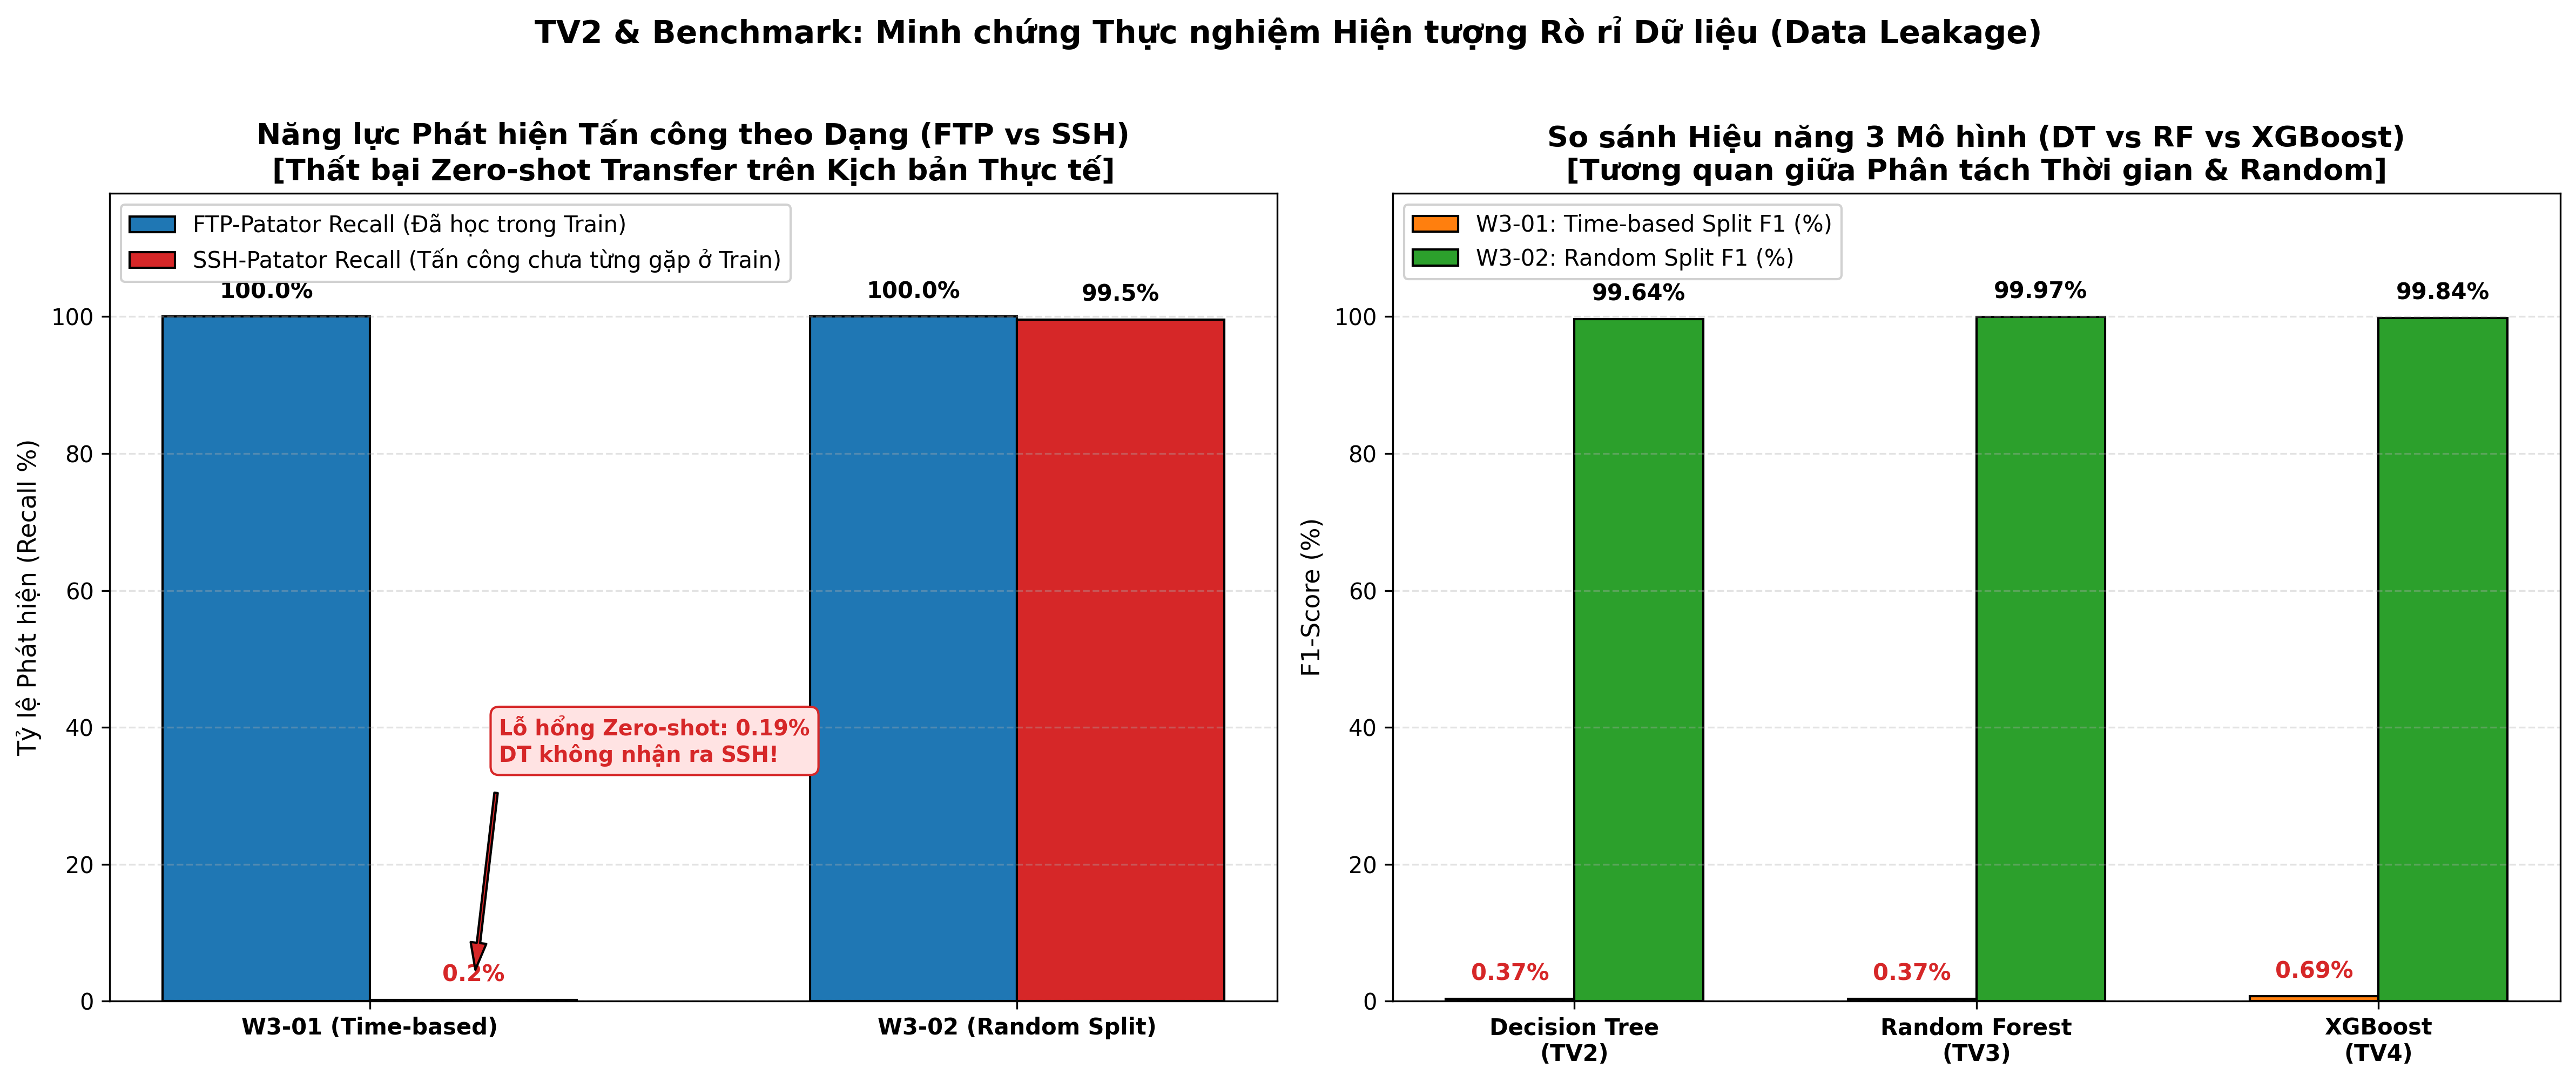
\includegraphics[width=0.92\textwidth]{experiments/figures/06_data_leakage_benchmark.png}
\caption{Đối chiếu hiệu năng giữa Random Split và Time-based Split; chênh lệch đồng thời phản ánh khác biệt về giao thức và thành phần subtype.}
\label{fig:data_leakage_benchmark}
\end{figure}

Kết quả này phù hợp với các phân tích của Arp và cộng sự \cite{arp2022dos} cũng như Pendlebury và cộng sự \cite{pendlebury2019tesseract}, theo đó chia ngẫu nhiên có thể tạo ra ước lượng lạc quan khi các mẫu phụ thuộc hoặc thuộc cùng chiến dịch xuất hiện ở nhiều tập. Trong thí nghiệm này, campaign-level dependence là một giải thích khả dĩ, nhưng chưa có bằng chứng trực tiếp về rò rỉ nhãn hay đặc trưng. Điểm số cao của Random Split không nên được diễn giải riêng như bằng chứng về khái quát hóa sang chiến dịch, subtype hoặc thời điểm mới; muốn cô lập tác động của chiến lược chia cần kiểm soát thành phần subtype và phân bố Test tương đương.
